\StartPlate{V15}{Equal weighted sums can conceal different capacity}{The conductor formula has already discarded the parity information needed for the quotient.}
\begin{center}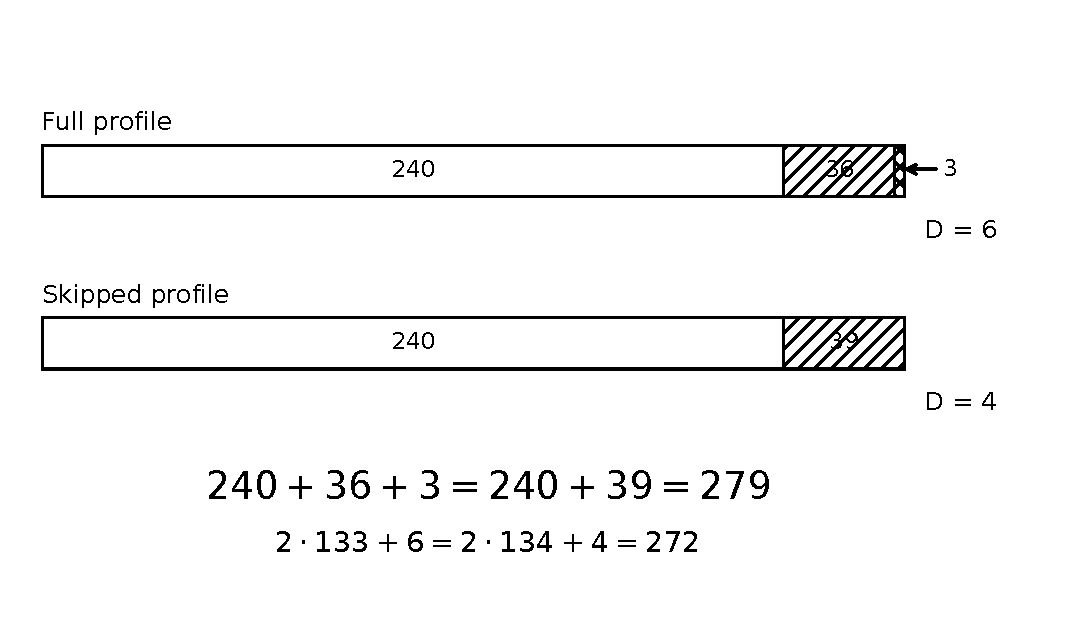
\includegraphics[width=\linewidth]{figures/V15.pdf}\end{center}
The full rank-eight profile has centralizer dimensions $(8,4,2,1)$ and levels $(60,18,3)$. The skipped profile has dimensions $(8,4,1)$ and levels $(60,13)$. The bar segments are the products $\Delta_j\nu_j$. Both sum to $279$, giving ordinary self-pair conductor $63+279=342$.
\[
(I,D)_{\rm full}=(133,6),\qquad (I,D)_{\rm skipped}=(134,4).
\]
The compensation $2\cdot133+6=2\cdot134+4$ explains the equality. The identity $2\lceil\nu/2\rceil+\mathbf1_{2\mid\nu}=\nu+1$ removes the parity distribution from the weighted conductor sum, while $D$ retains it.

Under their inherited arithmetic construction hypotheses, both profiles also have standard conductor $68$ and torsion number one. Yet only the full profile has room for the six-dimensional source quotient in this specified host. The new tests verify the grade consequences. They do not freshly construct the skipped-profile parameter or turn three agreeing integers into H5.
\vfill\PlateSource{Exact information-loss example}{Part III, Section 24}{62}
